\documentclass[10pt,twocolumn,letterpaper]{ctexart}
\usepackage{CJK}
\usepackage{graphicx}
\usepackage{subfigure}
\usepackage{cvpr}
\usepackage{float}
\usepackage{times}
\usepackage{epsfig}
\usepackage{graphicx}
\usepackage{amsmath}
\usepackage{amssymb}


\usepackage[breaklinks=true,bookmarks=false]{hyperref}

\cvprfinalcopy % *** Uncomment this line for the final submission

\setcounter{page}{1}
\usepackage{indentfirst}
\setlength{\parindent}{2em}
\begin{document}

%%%%%%%%% TITLE
\title{Efficient Gradient-Domain Compositing Using Quadtrees Experiment Report}

\author{2014011355\\
辛杭高}



\maketitle
%\thispagestyle{empty}

\begin{abstract}
   本次实验中,我实现了论文Efficient Gradient-Domain Compositing Using Quadtrees中的算法,能够完成图象融合工作。报告中我介绍了关于本算法的细节,在文末,我附上了一些本次实验的结果,并将实验的结果与
   未使用Quadtree的泊松融合算法进行了比较。
\end{abstract}

\section{泊松融合的思想及局限}
   图片融合的任务中,如果直接将原图的部分拷贝到目标图片中,会产生比较明显的融合边界。因为在融合边界处,图片的梯度是由人为因素造成的。为了增强融合后图片的真实性,该方法将融合区域的梯度修正为目标梯度,从而达到消除融合边界的效果。目标梯度的选取是多样的,可以选择原图像相应区域的梯度,也可以选择目标图像相应区域的梯度,还可以是两者的混合。

   以修改梯度为目标的思想可以转化为方程:
   \begin{equation}
      Ax = b
   \end{equation}
   其中x是融合区域各个像素组成的向量,b是目标梯度。为方便表述,我们用n来表示待融合区域
   像素的数目。A是用来求像素梯度的稀疏矩阵,规模为$n^2$,每一行仅有两个元素非零。

   这是一个过约束线性系统,因此在欧式距离的意义上减小Ax与b的差异,可转化为线性系统
   \begin{equation}
      AxA^{T} = A^{T}b
   \end{equation}

   在方程(2)里,Laplacian变化的每行最多有5个元素非零。在解方程的时候会有比较高的复杂度,这给泊松融合的时间和空间都
   带来很大的压力。利用Quadtree可以极大地减小矩阵A的规模,通常可以将$n * n$降低到$ \sqrt{n} *  \sqrt{n}$。

\section{优化的核心思想}
   对(1)中的x重新进行表述:
   \begin{equation}
      x = x_0 + x_\delta
   \end{equation}
   则(2)中的方程可以改写为:
   \begin{equation}
      A^{T}Ax_\delta = A^{T}(b-Ax_0)
   \end{equation}

   此时我们选择原图像的梯度作为b。显然,如果x的Laplacian变化不需要涉及到融合区域的边界,那么(4)式方程的右边为
   0。

   因此,对于融合区域的所有内部元素方程$ A^{T}Ax_\delta = 0$成立。此式子成立为双线性插值提供了支撑,保证了双线性
   插值的合理性。

   综上,我们只需要参照某种依据将待融合区域划分成Quadtree的子节点,在Quadtree的叶节点上进行双线性插值,即可解出
   待融合区域各像素点的RGB值。
\section{双线性插值}
   双线性插值是有两个变量的插值函数的线性插值扩展,其核心思想是在两个方向分别进行一次线性插值。红色的数据点与待插值得到的绿色点。假如我们想得到未知函数{$\displaystyle f$}在点{$\displaystyle P=\left(x,y\right)$}的值。
   假设我们已知函数{$\displaystyle f$}在{$\displaystyle Q_{11}=\left(x_1,y_1\right)$},{$\displaystyle Q_{12}=\left(x_1,y_2\right)$},{$\displaystyle Q_{21}=\left(x_2,y_1\right)$},{$\displaystyle Q_{22}=\left(x_2,y_2\right)$}四个点的值。

   \begin{figure}[t]
   \begin{center}
      \includegraphics[width=0.8\linewidth]{Bilinear.png}
   \end{center}
      \caption{红色的数据点与待插值得到的绿色点.}
   \label{fig:long}
   \label{fig:onecol}
   \end{figure}

   首先在x方向进行线性插值,得到
   \begin{equation}
   {\displaystyle f(R_{1})\approx {\frac {x_{2}-x}{x_{2}-x_{1}}}f(Q_{11})+{\frac {x-x_{1}}{x_{2}-x_{1}}}f(Q_{21})\quad R_{1}=(x,y_{1}),}
   \end{equation}

   \begin{equation}
   {\displaystyle f(R_{2})\approx {\frac {x_{2}-x}{x_{2}-x_{1}}}f(Q_{12})+{\frac {x-x_{1}}{x_{2}-x_{1}}}f(Q_{22})\quad R_{1}=(x,y_{2})。}
   \end{equation}

   然后在 y 方向进行线性插值,得到
   \begin{equation}
   {\displaystyle f(P)\approx {\frac {y_{2}-y}{y_{2}-y_{1}}}f(R_{1})+{\frac {y-y_{1}}{y_{2}-y_{1}}}f(R_{2}).}
   \end{equation}

   用矩阵运算表示为
   \begin{equation}
   {\displaystyle f(x,y)\approx {\begin{bmatrix}1-x&x\end{bmatrix}}{\begin{bmatrix}f(0,0)&f(0,1)\\f(1,0)&f(1,1)\end{bmatrix}}{\begin{bmatrix}1-y\\y\end{bmatrix}}}
   \end{equation}

\subsection{T-Junction}
   由上述定义可知,为了完成双线性插值的工作,除了以左上角的节点为基点之外,还需要引入右侧相邻叶节点的像素值和下方相邻
   叶节点的像素值。

   由于Quadtree的划分过程本身对子节点之间的关系并没有要求,因此对于某个叶节点来说,与其相邻的节点规模难以确定,致使
   我们无法求出右侧相邻节点和下方相邻节点的像素值。

   为了能够精确求出某叶节点右侧和正下方叶节点的像素值,我们规定某个节点与其相邻节点规模的差异不能超过两倍,否则需要进一
   步对Quadtree的划分进行细化。

   此时分为三种情况,若某叶节点的相邻节点与其规模相同,则显然不形成T-Junction。若相邻节点的规模是本节点的一半,那也不
   形成T-Junction,因为此时右侧节点和正下方节点的像素值可以直接获取。若相邻节点的规模是本节点的两倍,则此时形成T-Junction.

   对于T-Junction,其像素值需要通过相邻节点的插值得到,如此也可以保证插值的连续性。
   \begin{figure}[t]
   \begin{center}
      \includegraphics[width=1.0\linewidth]{Tjunction.jpeg}
   \end{center}
      \caption{箭头所指位置即为T-Junction,其像素值需要通过插值得到.}
   \label{fig:long}
   \label{fig:onecol}
   \end{figure}

\section{Quadtree 划分原则}
   双线性插值是以Quadtree的叶节点为基本单位的,因此我们划分Quadtree的首要依据是保证双线性插值的合理性。双线性插值
   只有在(4)式右侧为0时才合理,即必须使得需要被插值的叶节点内部不包含边界点。如果某个叶节点的规模为1,该节点
   就不需要进行插值,当然可以包含边界点。

   综上,我们对Quadtree是否还有必要进行划分的依据是:

   (1)该节点若包含边界点,则应该继续划分下去,直至不包含边界点或该节点的规模变为1。
   (2)节点划分的过程中,必须满足节点与相邻节点的规模差异不超过2倍,否则将形成除T-Junction之外的其他插值情况。

   另外,我们在插值过程中,会寻找每个节点的右侧节点与正下方节点,为保证这两者都存在,我们需要人为的规定,最右侧与最下方
   的一排像素点为边界点,以便使得会有某个叶节点单独包含它们。

   下图为某次实验中我们得到的Quadtree划分结果,其中每个正方形方块代表一个叶节点,每个叶节点的灰度值随机产生。从图中
   可以看出,在边界位置处,分布着密集的叶节点,在非边界位置,叶节点的数目明显减少。但是为了保证相邻节点之间的规模之差不会超过两倍,也不会产生过大的叶节点。

   如前所述,图象最右侧和最下方的一排像素都被人为设置成了边界点,以此来保证每个点在进行插值运算的时候可以找到需要的插值
   点,当然,如此会加大部分时间上的复杂度。
   \begin{figure}[t]
   \begin{center}
      \includegraphics[width=1.0\linewidth]{quadMat.png}
   \end{center}
      \caption{箭头所指位置即为T-Junction,其像素值需要通过插值得到.}
   \label{fig:long}
   \label{fig:onecol}
   \end{figure}
\subsection{边界点的寻找}
   在本任务中,我们会根据一张用来标记原图像的mask图象来寻找融合区域的边界位置。在mask图象中,0表示非融合区域,1表示融
   合区域。我们需要找的边界点由由待融合区域的最外层组成,该层像素点的相邻像素中至少有一个是非融合区域的像素。为了找到这
   些边界点,我们对mask图象进行一次卷积操作,卷积核为:

   \begin{equation}
   \begin{bmatrix}
   1 & 1 & 1\\
   1 & 1 & 1\\
   1 & 1 & 1
   \end{bmatrix}
   \end{equation}

   卷积后,若某点的值小于9则说明该点在边界范围内。
\section{降维后的泊松方程}
   在泊松方程的求解过程中,方程的维度由融合区域像素个数来决定。对于降维后的泊松方程,方程的维度由Quadtree的叶节点个数
   来决定。

   方程右侧的b向量,在未降维度的时候是由融合区域像素之间的差异来决定的,在降维后的情况下,向量由融合区域内叶节点之间像
   素的差异来决定。

   也正是由于此处降低了解方程的维度,最终解方程的时候才会大大缩短时间,从根本上讲缩短了进行图象融合的时间。

   设叶节点的数目为m,则时间和空间的复杂度会降低到O(m),通常情况下,$m = O(\sqrt{n})$。

   解出方程之后,即可得到各个节点的像素值。再根据各个点的像素值,来通过双线性插值来解出最后图象中的像素值。

   降维后的泊松方程求解即为法方程的求解:
   \begin{equation}
      S^T A^T A S S_\delta = S^T A^T (b - ASy_0)
   \end{equation}
   双线性插值的过程也可以表述为:
   \begin{equation}
      x = Sy
   \end{equation}

   \begin{figure}
   \centering
   \subfigure[用于融合的前景与背景]{
   \begin{minipage}[b]{0.4\textwidth}
   \includegraphics[width=1\textwidth]{fbg.jpg} \\
   \includegraphics[width=1\textwidth]{ffg.jpg}
   \end{minipage}
   }
   \end{figure}
   以上图为例,在降为前泊松融合的维度为44792,降为后仅为4732。
   
   \onecolumn
   一

   \begin{figure}[H]
     \centering
     \subfigure[原图像]{
       \label{fig:subfig:a} %% label for first subfigure
       \includegraphics[width=0.4\columnwidth]{ffg.jpg}}
     \hspace{1in}
     \subfigure[目标图象]{
       \label{fig:subfig:b} %% label for second subfigure
       \includegraphics[width=0.4\columnwidth]{fbg.jpg}}
     \caption{原图象和目标图象}
     \label{fig:subfig} %% label for entire figure
   \end{figure}

   \begin{figure}[H]
     \centering
     \subfigure[未降维泊松融合的结果]{
       \label{fig:subfig:a} %% label for first subfigure
       \includegraphics[width=0.45\columnwidth]{fnaive.png}}
     \hspace{1in}
     \subfigure[降维后泊松融合的结果]{
       \label{fig:subfig:b} %% label for second subfigure
       \includegraphics[width=0.45\columnwidth]{fquad.png}}
     \caption{降维和未降维后得到的结果}
     \label{fig:subfig} %% label for entire figure
   \end{figure}
   \clearpage
   一

   \begin{figure}[H]
     \centering
     \subfigure[原图像]{
       \label{fig:subfig:a} %% label for first subfigure
       \includegraphics[width=0.4\columnwidth]{wfg.jpg}}
     \hspace{1in}
     \subfigure[目标图象]{
       \label{fig:subfig:b} %% label for second subfigure
       \includegraphics[width=0.4\columnwidth]{wbg.jpg}}
     \caption{原图象和目标图象}
     \label{fig:subfig} %% label for entire figure
   \end{figure}

   \begin{figure}[H]
     \centering
     \subfigure[未降维泊松融合的结果]{
       \label{fig:subfig:a} %% label for first subfigure
       \includegraphics[width=0.4\columnwidth]{wnaive.png}}
     \hspace{1in}
     \subfigure[降维后泊松融合的结果]{
       \label{fig:subfig:b} %% label for second subfigure
       \includegraphics[width=0.4\columnwidth]{wquad.png}}
     \caption{降维和未降维后得到的结果}
     \label{fig:subfig} %% label for entire figure
   \end{figure}
   \clearpage

   一

   \begin{figure}[H]
     \centering
     \subfigure[原图像]{
       \label{fig:subfig:a} %% label for first subfigure
       \includegraphics[width=0.4\columnwidth]{pfg.jpg}}
     \hspace{1in}
     \subfigure[目标图象]{
       \label{fig:subfig:b} %% label for second subfigure
       \includegraphics[width=0.4\columnwidth]{pbg.jpg}}
     \caption{原图象和目标图象}
     \label{fig:subfig} %% label for entire figure
   \end{figure}

   \begin{figure}[H]
     \centering
     \subfigure[未降维泊松融合的结果]{
       \label{fig:subfig:a} %% label for first subfigure
       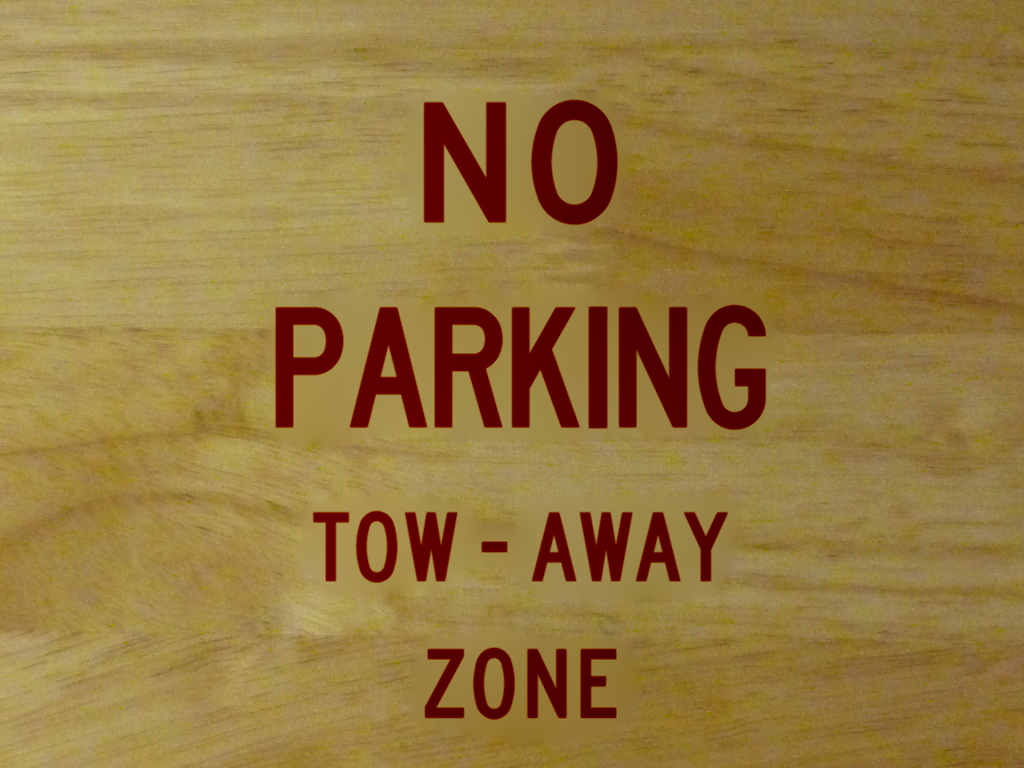
\includegraphics[width=0.4\columnwidth]{pnaive.png}}
     \hspace{1in}
     \subfigure[降维后泊松融合的结果]{
       \label{fig:subfig:b} %% label for second subfigure
       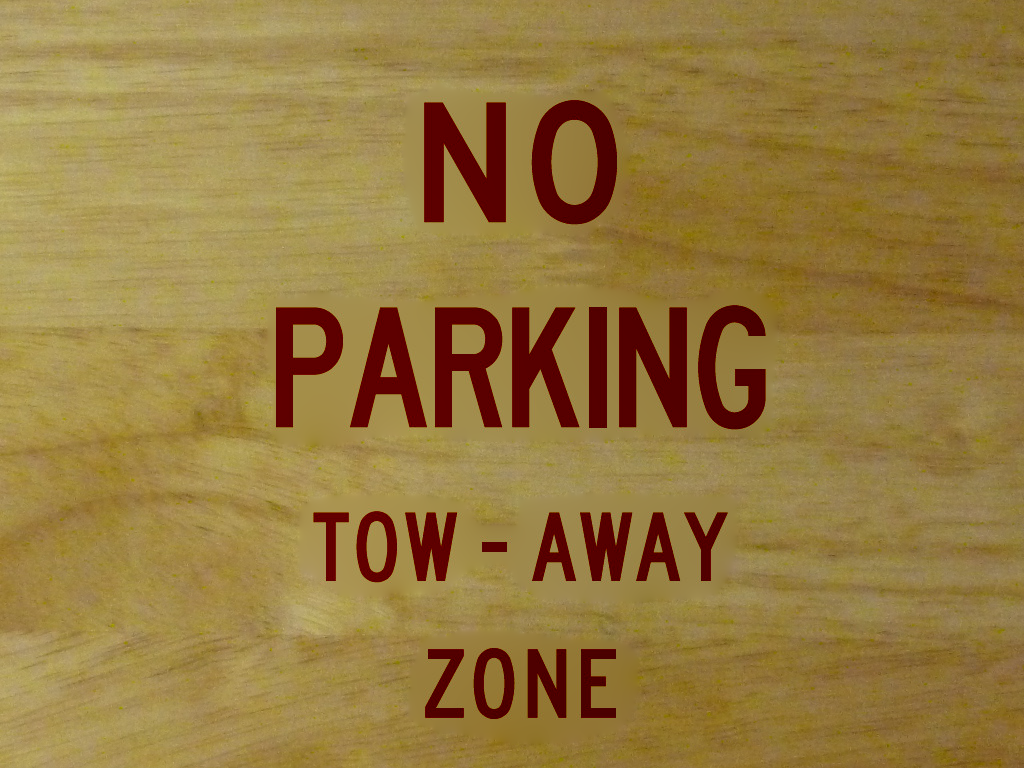
\includegraphics[width=0.4\columnwidth]{pquad.png}}
     \caption{降维和未降维后得到的结果}
     \label{fig:subfig} %% label for entire figure
   \end{figure}
   \clearpage

   一

   \begin{figure}[H]
     \centering
     \subfigure[原图像]{
       \label{fig:subfig:a} %% label for first subfigure
       \includegraphics[width=0.35\columnwidth]{mfg.jpg}}
     \hspace{1in}
     \subfigure[目标图象]{
       \label{fig:subfig:b} %% label for second subfigure
       \includegraphics[width=0.35\columnwidth]{mbg.jpg}}
     \caption{原图象和目标图象}
     \label{fig:subfig} %% label for entire figure
   \end{figure}

   \begin{figure}[H]
     \centering
     \subfigure[未降维泊松融合的结果]{
       \label{fig:subfig:a} %% label for first subfigure
       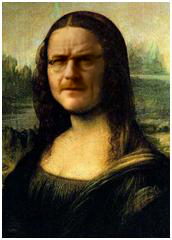
\includegraphics[width=0.4\columnwidth]{mnaive.png}}
     \hspace{1in}
     \subfigure[降维后泊松融合的结果]{
       \label{fig:subfig:b} %% label for second subfigure
       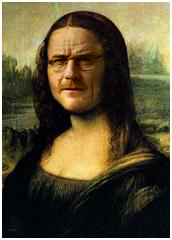
\includegraphics[width=0.4\columnwidth]{mquad.png}}
     \caption{降维和未降维后得到的结果}
     \label{fig:subfig} %% label for entire figure
   \end{figure}
   \clearpage
\end{document}
